% -----------------------------------------------------------------------------
% ------------------------------- The Preamble --------------------------------
% -----------------------------------------------------------------------------
% This is where you tell LaTeX how to render the document, import any external 
% packages you want to use (like amsmath), and declare custom commands.
% Note: much of the preamble of this document was forked from Professor Zajj 
% Daugherty. 

% This line tells LaTeX what style to use to render the document.
\documentclass[11pt, reqno]{amsart}

% Packages --------------------------------------------------------------------
% This is where you add whatever packages you need.
\usepackage[parfill]{parskip}          % Starts paragraphs with empty line
\usepackage{amsfonts, amscd, amssymb, amsthm, amsmath} % math packages
\usepackage{pdfsync}                   % leaves makers for tex searching
\usepackage{enumerate}				   % Set the style of item names
\usepackage{tikz}					   % For drawing graphs
\usetikzlibrary{arrows}
\usetikzlibrary{shapes}
\usepackage{biblatex}
% \usepackage[margin=1in]{geometry}    % Gives pages smaller margins (1in)   

% Theorem Environments -------------------------------------------------------- 
\theoremstyle{plain}
	\newtheorem{thm}{Theorem}[section]
	\newtheorem{lemma}[thm]{Lemma}
	\newtheorem{prop}[thm]{Proposition}
	\newtheorem{cor}[thm]{Corollary}
\theoremstyle{definition}
	\newtheorem*{defn}{Definition}
	\newtheorem{remark}[thm]{Remark}
\theoremstyle{example}
	\newtheorem*{example}{Example}

% Alphabets -------------------------------------------------------------------
%%% Some shortcuts for my commonly used special alphabets and characters.
\def\cA{\mathcal{A}}\def\cB{\mathcal{B}}\def\cC{\mathcal{C}}\def\cD{\mathcal{D}}\def\cE{\mathcal{E}}\def\cF{\mathcal{F}}\def\cG{\mathcal{G}}\def\cH{\mathcal{H}}\def\cI{\mathcal{I}}\def\cJ{\mathcal{J}}\def\cK{\mathcal{K}}\def\cL{\mathcal{L}}\def\cM{\mathcal{M}}\def\cN{\mathcal{N}}\def\cO{\mathcal{O}}\def\cP{\mathcal{P}}\def\cQ{\mathcal{Q}}\def\cR{\mathcal{R}}\def\cS{\mathcal{S}}\def\cT{\mathcal{T}}\def\cU{\mathcal{U}}\def\cV{\mathcal{V}}\def\cW{\mathcal{W}}\def\cX{\mathcal{X}}\def\cY{\mathcal{Y}}\def\cZ{\mathcal{Z}}
\def\AA{\mathbb{A}} \def\BB{\mathbb{B}} \def\CC{\mathbb{C}} \def\DD{\mathbb{D}} \def\EE{\mathbb{E}} \def\FF{\mathbb{F}} \def\GG{\mathbb{G}} \def\HH{\mathbb{H}} \def\II{\mathbb{I}} \def\JJ{\mathbb{J}} \def\KK{\mathbb{K}} \def\LL{\mathbb{L}} \def\MM{\mathbb{M}} \def\NN{\mathbb{N}} \def\OO{\mathbb{O}} \def\PP{\mathbb{P}} \def\QQ{\mathbb{Q}} \def\RR{\mathbb{R}} \def\SS{\mathbb{S}} \def\TT{\mathbb{T}} \def\UU{\mathbb{U}} \def\VV{\mathbb{V}} \def\WW{\mathbb{W}} \def\XX{\mathbb{X}} \def\YY{\mathbb{Y}} \def\ZZ{\mathbb{Z}}  
\def\fa{\mathfrak{a}} \def\fb{\mathfrak{b}} \def\fc{\mathfrak{c}} \def\fd{\mathfrak{d}} \def\fe{\mathfrak{e}} \def\ff{\mathfrak{f}} \def\fg{\mathfrak{g}} \def\fh{\mathfrak{h}} \def\fj{\mathfrak{j}} \def\fk{\mathfrak{k}} \def\fl{\mathfrak{l}} \def\fm{\mathfrak{m}} \def\fn{\mathfrak{n}} \def\fo{\mathfrak{o}} \def\fp{\mathfrak{p}} \def\fq{\mathfrak{q}} \def\fr{\mathfrak{r}} \def\fs{\mathfrak{s}} \def\ft{\mathfrak{t}} \def\fu{\mathfrak{u}} \def\fv{\mathfrak{v}} \def\fw{\mathfrak{w}} \def\fx{\mathfrak{x}} \def\fy{\mathfrak{y}} \def\fz{\mathfrak{z}}
\def\GL{\mathrm{GL}} \def\SL{\mathrm{SL}}  

\def\<{\langle} \def\>{\rangle}
\def\Aut{\mathrm{Aut}}
\def\dim{\mathrm{dim}} 
\def\End{\mathrm{End}} 
\def\ev{\mathrm{ev}} 
\def\img{\mathrm{img}}
\def\Hom{\mathrm{Hom}} 
\def\Fn{\mathrm{Fn}} 
\def\Fr{\mathcal{F}\mathrm{r}}
\def\id{\mathrm{id}} 
\def\sgn{\mathrm{sgn}}

% Bibliography management -----------------------------------------------------
\addbibresource{sample.bib}

% -----------------------------------------------------------------------------
% ------------------------------- The Document --------------------------------
% -----------------------------------------------------------------------------
% This is where you put everything you want to render on the PDF.
\begin{document}

% Document basics -------------------------------------------------------------
% This is how to make a title for your document.
\title{LaTeX Worksheet}
\author{CCNY AWM}
\maketitle

% These are some basic document organizing commands. 
\section{Section Title}
\subsection{Subsection Title}
Some plain text. 
\textit{Some italic text.}
\textbf{Some bold text.}

% A numbered list.
\begin{enumerate}[a)]
	\item The first item.
	\item The second item.
\end{enumerate}

% A bullet point list. 
\begin{itemize}
	\item The first item. 
	\item The second item
\end{itemize}

% A basic table:
\begin{center}
	\begin{tabular}{ | c || c | c | } \hline
			 & col1  & col2  \\ \hline \hline
		row1 & cell1 & cell2 \\ \hline 
		row2 & cell3 & cell4 \\ \hline
	\end{tabular}
\end{center}

% importing a photo 
TODO

% Drawing diagrams with tikz --------------------------------------------------
% The following code might seem complicated at first, but it's really just 
% a set of rules that tells tikz two things: 1) where to put a node and 2) where 
% to put an arrow. Everything else is style on those two things. Don't forget
% your semicolons!  
% 	\node (B) at (-1.25, 0) {$\cB$};
% means "create a new node called B at these coordinates, and give it the label 
% $\cB$" and 
%   \draw[->] (B)   -- node[above] {incl}      (FrB);
% means "draw an arrow from B to FrB, and label it above the line with 'incl'".  

\begin{figure}[htbp]
	\centering 
	$$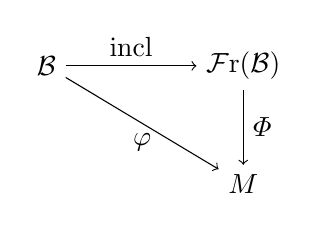
\begin{tikzpicture}
		\node (B)   at (-1.25, 0)   {$\cB$};
		\node (FrB) at (1.25, 0)    {$\Fr(\cB)$};
		\node (M)   at (1.25, -1.5) {$M$};
			
		\draw[->] (B)   -- node[above] {incl}      (FrB);
		\draw[->] (FrB) -- node[right] {$\varPhi$} (M);
		\draw[->] (B)   -- node[below] {$\varphi$} (M);
	\end{tikzpicture}$$ 
	\caption{The universal property of free modules. (This diagram commutes!)}
\end{figure}


% Using theorem environments --------------------------------------------------
% Some useful math environments based on the amsmath and amsthm packages. You 
% need to define these environments before you use them, as above. Then you can 
% use them like this:
\begin{thm}[Theorem Name]
	Theorem statement.
\end{thm}

\begin{proof}
	A Proof.
\end{proof}

\begin{defn}[Term]
	Definition statement.
\end{defn}


% ---------------------------------------------------------------------------
% -------------------------------- Math Mode --------------------------------
% ---------------------------------------------------------------------------
% For a fairly complete list of useful math mode symbols, see
% https://www.caam.rice.edu/~heinken/latex/symbols.pdf

% Inline math environment.
Here's an inline math equation: $f: X \rightarrow Y$. 

% New line math environment, two ways.
$$g: X \rightarrow Y$$
\[h: X \rightarrow Y\]

% Lining up several equations.
\begin{align*}
  (a + b) + (c + d) &= ((a + b) + c) + d \\
  &= (a + (b + c)) + d \\ 
  &= a + ((b + c) + d) \\ 
  &= a + (b + (c + d)) 
\end{align*}

% Numbering an equation
\begin{align}
	||a+b|| \leq ||a|| + ||b||
\end{align}

% A matrix
\[\begin{pmatrix}
	1 & 0 & 0 \\ 
	0 & 1 & 0 \\ 
	0 & 0 & 1 \\
\end{pmatrix}\]

% Piecewise function (requires amsmath package)
\[ f(x) = 
\begin{cases} 
	1, &\text{x rational } \\
	0, &\text{x irrational}	
\end{cases}
\]

% Delimiters that match the size of whatever is in them
\[det(A) = \sum_{\sigma \in S_n}\text{sgn}(\sigma)\left(\prod_{i=1}^n \alpha_{i, \sigma(i)}\right)\]

% ---------------------------------------------------------------------------
% ------------------------------ Bibliography -------------------------------
% ---------------------------------------------------------------------------
% This document manages the bibliography with the biblatex package. 
% Your sources are declared in another file, and then imported in the 
% preamble, like we've done with sample.bib. 
% You can then cite a source like this. 
Here's an article citation. \cite{vershik}
Here's a book citation with a specific section. \cite[\S 1.1]{riehl}
Here's a website citation. \cite{wiki-tensor}

% And display the bibliography at the end.
\printbibliography

% See Overleaf's guide for different ways of citing resources:
% https://www.overleaf.com/learn/latex/Bibliography_management_in_LaTeX#Reference_guide

% Every environment has to end like this
\end{document}

% ---------------------------------------------------------------------------
% ----------------------------- More References -----------------------------
% ---------------------------------------------------------------------------
% What goes into a LaTeX document:
%   https://en.wikibooks.org/wiki/LaTeX/Document_Structure
%
% Math related LaTeX packages and symbols:
%   https://en.wikibooks.org/wiki/LaTeX/Mathematics
%   https://en.wikibooks.org/wiki/LaTeX/Advanced_Mathematics
%   https://en.wikibooks.org/wiki/LaTeX/Theorems
% 
% Using a bibliography: 
%   https://www.overleaf.com/learn/latex/Bibliography_management_in_LaTeX#Reference_guide
%   https://en.wikibooks.org/wiki/LaTeX/Bibliography_Management
% 
% Using TikZ:
% TODO

